% (find-LATEX "2021-1-C2-coisas-antigas.tex")
% (defun c () (interactive) (find-LATEXsh "lualatex -record 2021-1-C2-coisas-antigas.tex" :end))
% (defun C () (interactive) (find-LATEXsh "lualatex 2021-1-C2-coisas-antigas.tex" "Success!!!"))
% (defun D () (interactive) (find-pdf-page      "~/LATEX/2021-1-C2-coisas-antigas.pdf"))
% (defun d () (interactive) (find-pdftools-page "~/LATEX/2021-1-C2-coisas-antigas.pdf"))
% (defun e () (interactive) (find-LATEX "2021-1-C2-coisas-antigas.tex"))
% (defun o () (interactive) (find-LATEX "2021-1-C2-coisas-antigas.tex"))
% (defun u () (interactive) (find-latex-upload-links "2021-1-C2-coisas-antigas"))
% (defun v () (interactive) (find-2a '(e) '(d)))
% (defun d0 () (interactive) (find-ebuffer "2021-1-C2-coisas-antigas.pdf"))
% (defun cv () (interactive) (C) (ee-kill-this-buffer) (v) (g))
%          (code-eec-LATEX "2021-1-C2-coisas-antigas")
% (find-pdf-page   "~/LATEX/2021-1-C2-coisas-antigas.pdf")
% (find-sh0 "cp -v  ~/LATEX/2021-1-C2-coisas-antigas.pdf /tmp/")
% (find-sh0 "cp -v  ~/LATEX/2021-1-C2-coisas-antigas.pdf /tmp/pen/")
%     (find-xournalpp "/tmp/2021-1-C2-coisas-antigas.pdf")
%   file:///home/edrx/LATEX/2021-1-C2-coisas-antigas.pdf
%               file:///tmp/2021-1-C2-coisas-antigas.pdf
%           file:///tmp/pen/2021-1-C2-coisas-antigas.pdf
% http://angg.twu.net/LATEX/2021-1-C2-coisas-antigas.pdf
% (find-LATEX "2019.mk")
% (find-CN-aula-links "2021-1-C2-coisas-antigas" "2" "c2m211ca" "c2ca")
%
% Video (not yet):
% (find-ssr-links "c2m211ca" "2021-1-C2-coisas-antigas")
% (code-video     "c2m211cavideo" "$S/http/angg.twu.net/eev-videos/2021-1-C2-coisas-antigas.mp4")
% (find-c2m211cavideo "0:00")

% «.defs»	(to "defs")
% «.title»	(to "title")
%
% «.djvuize»	(to "djvuize")

\documentclass[oneside,12pt]{article}
\usepackage[colorlinks,citecolor=DarkRed,urlcolor=DarkRed]{hyperref} % (find-es "tex" "hyperref")
\usepackage{amsmath}
\usepackage{amsfonts}
\usepackage{amssymb}
\usepackage{pict2e}
\usepackage[x11names,svgnames]{xcolor} % (find-es "tex" "xcolor")
\usepackage{colorweb}                  % (find-es "tex" "colorweb")
%\usepackage{tikz}
%
% (find-dn6 "preamble6.lua" "preamble0")
%\usepackage{proof}   % For derivation trees ("%:" lines)
%\input diagxy        % For 2D diagrams ("%D" lines)
%\xyoption{curve}     % For the ".curve=" feature in 2D diagrams
%
\usepackage{edrx21}               % (find-LATEX "edrx21.sty")
\input edrxaccents.tex            % (find-LATEX "edrxaccents.tex")
\input edrxchars.tex              % (find-LATEX "edrxchars.tex")
\input edrxheadfoot.tex           % (find-LATEX "edrxheadfoot.tex")
\input edrxgac2.tex               % (find-LATEX "edrxgac2.tex")
%
%\usepackage[backend=biber,
%   style=alphabetic]{biblatex}            % (find-es "tex" "biber")
%\addbibresource{catsem-slides.bib}        % (find-LATEX "catsem-slides.bib")
%
% (find-es "tex" "geometry")
\usepackage[a6paper, landscape,
            top=1.5cm, bottom=.25cm, left=1cm, right=1cm, includefoot
           ]{geometry}
%
\begin{document}

\catcode`\^^J=10
\directlua{dofile "dednat6load.lua"}  % (find-LATEX "dednat6load.lua")

%L dofile "edrxtikz.lua"  -- (find-LATEX "edrxtikz.lua")
%L dofile "edrxpict.lua"  -- (find-LATEX "edrxpict.lua")
\pu

% «defs»  (to ".defs")
% (find-LATEX "edrx15.sty" "colors-2019")
%\long\def\ColorRed   #1{{\color{Red1}#1}}
%\long\def\ColorViolet#1{{\color{MagentaVioletLight}#1}}
%\long\def\ColorViolet#1{{\color{Violet!50!black}#1}}
%\long\def\ColorGreen #1{{\color{SpringDarkHard}#1}}
%\long\def\ColorGreen #1{{\color{SpringGreenDark}#1}}
%\long\def\ColorGreen #1{{\color{SpringGreen4}#1}}
%\long\def\ColorGray  #1{{\color{GrayLight}#1}}
%\long\def\ColorGray  #1{{\color{black!30!white}#1}}
%\long\def\ColorBrown #1{{\color{Brown}#1}}
%\long\def\ColorBrown #1{{\color{brown}#1}}
%\long\def\ColorOrange#1{{\color{orange}#1}}
%
%\long\def\ColorShort #1{{\color{SpringGreen4}#1}}
%\long\def\ColorLong  #1{{\color{Red1}#1}}
%
%\def\frown{\ensuremath{{=}{(}}}
%\def\True {\mathbf{V}}
%\def\False{\mathbf{F}}
%\def\D    {\displaystyle}

\def\mname#1{\text{[#1]}}

\def\drafturl{http://angg.twu.net/LATEX/2021-1-C2.pdf}
\def\drafturl{http://angg.twu.net/2021.1-C2.html}
\def\draftfooter{\tiny \href{\drafturl}{\jobname{}} \ColorBrown{\shorttoday{} \hours}}



%  _____ _ _   _                               
% |_   _(_) |_| | ___   _ __   __ _  __ _  ___ 
%   | | | | __| |/ _ \ | '_ \ / _` |/ _` |/ _ \
%   | | | | |_| |  __/ | |_) | (_| | (_| |  __/
%   |_| |_|\__|_|\___| | .__/ \__,_|\__, |\___|
%                      |_|          |___/      
%
% «title»  (to ".title")
% (c2m211cap 1 "title")
% (c2m211caa   "title")

\thispagestyle{empty}

\begin{center}

\vspace*{1.2cm}

{\bf \Large Cálculo 2 - 2021.1}

\bsk

Slides de 2020.1 e 2020.2

que eu posso querer reusar

\bsk

Eduardo Ochs - RCN/PURO/UFF

\url{http://angg.twu.net/2021.1-C2.html}

\end{center}

\newpage




% «exemplao»  (to ".exemplao")
% (c2m211somas2p 27 "exemplao")
% (c2m211somas2a    "exemplao")

{\bf Exemplão: métodos do sup e do inf}

\long\def\ColorUpper #1{{\color{red!20!white}#1}}
\long\def\ColorUpperB#1{{\color{red!30!white}#1}}
\long\def\ColorLower #1{{\color{red!40!white}#1}}
\long\def\ColorLowerB#1{{\color{red!50!white}#1}}

\msk

%\phantom{a}

%\vspace*{-1cm}

Seja
$f(x)=
    \unitlength=10pt
    \celllower=2.5pt%
    \def\cellfont{\scriptsize}%
    %
    \vcenter{\hbox{%
    \beginpicture(0,0)(5,6)
    \pictgrid%
    \ColorUpper {\polygon*(1,5)(3,5)(3,0)(1,0)}%
    \ColorUpperB{\polygon (1,5)(3,5)(3,0)(1,0)}%
    \ColorLower {\polygon*(1,1)(3,1)(3,0)(1,0)}%
    \ColorLowerB{\polygon (1,1)(3,1)(3,0)(1,0)}%
    \pictpiecewise{(0,3)--(2,5)o (2,3)c (2,1)o--(5,4)}%
    %\put(3,6.25){\cell{(3,6)}}%
    %\put(8,0.75){\cell{(8,1)}}%
    \pictaxes%
    \ColorRed{%
      %\linethickness{4pt}
      \pictpiecewise{(1,0)c--(3,0)c
                     (1,4)c--(2,5)o (2,3)c (2,1)o--(3,2)c
                     (0,4)c--(0,5)o (0,3)c (0,1)o--(0,2)c
                    }%
    }
    \end{picture}%
    }}
    =
    \scalebox{1.0}{$
    \begin{cases}
    x+3 & \text{quando $x<2$}, \\
    3   & \text{quando $x=2$}, \\
    x-1 & \text{quando $2<x$}. \\
    \end{cases}
    $}
   $

\msk

$\begin{array}{lrcl}
 \text{Seja}  &        B   &=& [1,3]. \\
 \text{Então} &      F(B)  &=& (1,2)∪\{3\}∪[4,5), \\
              &    U(F(B)) &=& [5,+∞], \\
              &    L(F(B)) &=& [-∞,1], \\
              & \sup(F(B)) &=& 5, \\
              & \inf(F(B)) &=& 1, \\
 \end{array}
$

\msk

$\sup(F([1,3]))·(3-1) $ é o retângulo mais claro, 

$\inf(F([1,3]))·(3-1) $ é o retângulo mais escuro... 



\newpage

% «exercicio-10»  (to ".exercicio-10")
% (c2m211somas2p 20 "exercicio-10")
% (c2m211somas2a    "exercicio-10")

% {\bf Exercício 10.}
% 
% \ssk
% 
% Seja:
% 
% $f(x)=
%     \unitlength=10pt
%     \celllower=2.5pt%
%     \def\cellfont{\scriptsize}%
%     %
%     \vcenter{\hbox{%
%     \beginpicture(0,0)(11,7)
%     \pictgrid%
%     \pictpiecewise{(0,3)--(3,6)--(8,1)--(11,4)}%
%     \put(3,6.5){\cell{(3,6)}}%
%     \put(8,0.5){\cell{(8,1)}}%
%     \pictaxes%
%     \end{picture}%
%     }}
%     =
%     \scalebox{1.0}{$
%     \begin{cases}
%     x+3 & \text{quando $x≤3$}, \\
%     9-x & \text{quando $3<x<8$}, \\
%     x-7 & \text{quando $8≤x$} \\
%     \end{cases}
%     $}
%    $
% 
% \msk
% 
% Seja $P = \{1,2,4,5,7,9,10\}$.
% 
% Represente graficamente:
% 
% \ssk
% 
% a) $\sum_{i=1}^{N} \inf(F([a_i,b_i]))·(b_i-a_i)$
% 
% b) $\sum_{i=1}^{N} \sup(F([a_i,b_i]))·(b_i-a_i)$
% 
% Dica: represente o (a) e o (b) no mesmo gráfico usando retângulos de
% cores diferentes, como nas figuras das páginas 2 e 19.
% 
% \newpage

% «intover-intunder»  (to ".intover-intunder")
% (c2m211somas2p 21 "intover-intunder")
% (c2m211somas2a    "intover-intunder")

% {\bf Aproximações por cima e por baixo}
% 
% \ssk
% 
% Na aula 1 nós vimos esta figura:
% 
% $$\Intx{a}{b}{f(x)} = \Area \left(
%   \myvcenter{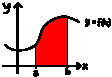
\includegraphics[width=2cm]{2020-1-C2/area-intro-1.pdf}}
%   \right)
% $$
% 
% As aproximações da integral de $f$ por retângulos por cima e por baixo
% dependem da escolha de uma partição $P$ do intervalo $[a,b]$. As
% definições formais são:
% %

\def\Intover #1#2{\overline {∫}_{#1}#2\,dx}
\def\Intunder#1#2{\underline{∫}_{#1}#2\,dx}
\def\Intoverunder#1#2{\Intover{#1}{#2} - \Intunder{#1}{#2}}
%
\def\Intxover #1#2#3{\overline {∫}_{x=#1}^{x=#2}#3\,dx}
\def\Intxunder#1#2#3{\underline{∫}_{x=#1}^{x=#2}#3\,dx}

% %
% $$\begin{array}{rcl}
%   \D \Intover {P}{f(x)} &=& \sum_{i=1}^{N} \sup(F([a_i,b_i]))·(b_i-a_i) \\[12pt]
%   \D \Intunder{P}{f(x)} &=& \sum_{i=1}^{N} \inf(F([a_i,b_i]))·(b_i-a_i) \\
%   \end{array}
% $$



% \newpage
% 
% % «exercicio-11»  (to ".exercicio-11")
% 
% {\bf Exercício 11.}
% 
% \ssk
% 
% Seja $f(x)$ a função do exercício 10.
% 
% Seja $P = \{1, 2, 3, \ldots, 10\}$.
% 
% Represente graficamente (num gráfico só)
% %
% $$f(x), \quad \D \Intunder {P}{f(x)}, \quad \D \Intover {P}{f(x)}.$$
% 
% A diferença entre as duas aproximações, $\D \Intover {P}{f(x)} - \D \Intunder {P}{f(x)}$,
% 
% corresponde à área em rosa claro nos slides 2 e 19.
% 
% Ela consiste num certo número de quadrados $1×1$.
% 
% \ColorRed{Quantos?}
% 
% \newpage
% 
% % «exercicio-12»  (to ".exercicio-12")
% % (c2m211somas2p 23 "exercicio-12")
% % (c2m211somas2a    "exercicio-12")
% 
% {\bf Exercício 12.}
% 
% \ssk
% 
% Faça a mesma coisa, mas agora para a partição
% 
% $P = \{1, 1.5, 2, 2.5, \ldots, 10\}$.
% 
% \ssk
% 
% Agora a diferença $\D \Intover {P}{f(x)} - \D \Intunder {P}{f(x)}$
% 
% \ssk
% 
% é feita de um certo número de quadrados
% 
% de dimensões $0.5×0.5$.
% 
% \ColorRed{Quantos?}
% 
% 
% \newpage
% 
% % «exercicio-13»  (to ".exercicio-13")
% % (c2m211somas2p 24 "exercicio-13")
% % (c2m211somas2a    "exercicio-13")
% 
% {\bf Exercício 13.}
% 
% \ssk
% 
% Sejam:
% 
% $f(x) = 4 - (x-2)^2$,
% 
% $P_0 = \{0,4\}$,
% 
% $P_1 = \{0,2,4\}$,
% 
% $P_2 = \{0,1,2,3,4\}$,
% 
% $P_3 = \{0,0.5,1,1.5, \ldots, 4\}$.
% 
% a) Represente graficamente $\D \Intover {P_3}{f(x)} - \D \Intunder {P_3}{f(x)}$.
% 
% \newpage
% 
% {\bf Exercício 13 (cont.)}
% 
% \ssk
% 
% b) Represente \ColorRed{num gráfico só}:
% 
% $\Intx{0}{4}{f(x)}$,
% 
% $\Intoverunder {P_0}{f(x)}$,
% 
% $\Intoverunder {P_1}{f(x)}$,
% 
% $\Intoverunder {P_2}{f(x)}$,
% 
% $\Intoverunder {P_3}{f(x)}$.
% 
% \msk
% 
% c) Seja $A = \Intoverunder {P_3}{f(x)}$, considerado como um
% subconjunto de $\R^2$ formado de retângulos, e $B$ o conjunto obtido a
% partir de $A$ deslizando cada retângulo de $A$ pra baixo como
% explicado no vídeo. Desenhe $B$ direito e obtenha uma estimativa para
% a área de $B$ seguindo as idéias do vídeo.

\newpage

{\bf Exercício 13 (cont.)}

\ssk

d) Faça a mesma coisa que no item c, mas usando a partição $P_4$.

Você deve obter algo desta forma:
%
$$0 \le \Area(
  % (find-latexscan-links "C2" "20210225_retangulinhos")
  \myvcenter{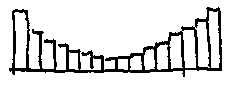
\includegraphics[height=0.5cm]{2020-2-C2/20210225_retangulinhos.pdf}}
  ) \le \_\_,
$$

onde o ``$\_\_$'' é ou um número ou uma expressão fácil de calcular.

\msk

e) Faça a mesma coisa que no item d, mas usando a partição $P_5$.

f) Faça a mesma coisa que no item d, mas usando a partição $P_6$.




\newpage

{\bf Exercício 14.}

\ssk

Repare que dá pra expressar a partição que divide o intervalo

$[a,b]$ em $N$ partes iguais assim:
%
$$\{a, \; a+1·\frac{b-a}{N},
       \; a+2·\frac{b-a}{N}, \ldots,
       \; a+N·\frac{b-a}{N}\}
$$

a) Teste a fórmula acima para o caso $[a,b]=[2,5]$, $N=6$.

b) Teste a fórmula acima para o caso $[a,b]=[2,5]$, $N=7$.

\msk

Dica importante: no Ensino Médio os professores dizem pra sempre fazer
``simplificações'' como esta aqui: $2 + 4·\frac{5-2}{7} =
\frac{26}{7}$. Em casos como a acima essas ``simplificações'' fazem
com que os padrões fiquem muito mais difíceis de entender.
\ColorRed{Não seja como aqueles professores do Ensino Médio!}

\newpage

% {\bf Exercício 14 (cont.)}
% 
% \ssk
% 
% Se estamos tentando integrar uma função no intervalo $[a,b]$
% 
% a nossa \ColorRed{sequência preferida de partições} para este
% intervalo
% 
% vai ser definida por:
% %
% $$P_k = \{ a, \; a + 1·\frac{b-a}{2^k}, \; a + 2·\frac{b-a}{2^k}, \ldots, b \}$$
% 
% 
% c) A partição $P_0$ tem quantos intervalos? E quantos pontos?
% 
% d) A partição $P_1$ tem quantos intervalos? E quantos pontos?
% 
% e) A partição $P_2$ tem quantos intervalos? E quantos pontos?
% 
% f) A partição $P_5$ tem quantos intervalos? E quantos pontos?
% 
% \newpage
% 
% {\bf Mais definições}
% 
% \ssk
% 
% Defs:
% %
% $$\begin{array}{rcl}
%   \D \Intxover {a}{b}{f(x)} &=& \D \lim_{k→∞} \Intover{P_k}{f(x)} \text{ e} \\[16pt]
%   \D \Intxunder{a}{b}{f(x)} &=& \D \lim_{k→∞} \Intunder{P_k}{f(x)}, \\
%   \end{array}
% $$
% 
% onde $P_0, P_1, P_2, P_3, \ldots$ é a nossa sequência preferida de
% partições
% 
% para o intervalo $[a,b]$, que definimos no slide anterior.
% 
% \newpage
% 
% {\bf Exercício 15.}
% 
% \ssk
% 
% Seja $f(x) = 4 - (x-2)^2$.
% 
% a) Represente graficamente $\Intxover {0}{4}{f(x)}$, representando
% 
% todas as ``$\Intover{P_k}{f(x)}$''s num gráfico só.
% 
% b) Represente graficamente $\Intxunder {0}{4}{f(x)}$, representando
% 
% todas as ``$\Intunder{P_k}{f(x)}$''s num gráfico só.
% 



\newpage

% «pierluigi»  (to ".pierluigi")
% (c2m211somas2p 34 "pierluigi")
% (c2m211somas2a    "pierluigi")
% (find-books "__analysis/__analysis.el" "beneveri")

{\bf As notas do Pierluigi Benevieri}

\ssk

Agora dê uma olhada nestas notas

de Cálculo 2 do Pierluigi Benevieri:

\ssk

\url{https://www.ime.usp.br/~pluigi/registro-MAT121-15.pdf}

\ssk

Nas páginas 3 e 4 ele define a integral (na definição 3) usando a
``família de todas as partições do intervalo $[a,b]$''... isto é
beeeem mais difícil de entender e visualizar do que o que eu fiz aqui,
usando o limite na minha sequência preferida de partições do intervalo
$[a,b]$...

\newpage

% {\bf Exercício 16.}
% 
% \ssk
% 
% a) Entenda a definição da Função de Dirichlet que o Pierluigi faz nas
% páginas 8 e 9, e que ele chama de $f(x)$ naquele trecho das notas.
% 
% b) Faça o gráfico dessa função $f(x)$.
% 
% \msk
% 
% Seja $[a,b]=[2,5]$.
% 
% c) Represente graficamente $\Intover{P_k}{f(x)}$ e
% $\Intunder{P_k}{f(x)}$
% 
% para $k=0$, $k=1$ e $k=2$.
% 
% d) Convença-se de que 
% %
% $$\Intxover {2}{5}{f(x)} = 3 \quad \text{e} \quad
%   \Intxunder{2}{5}{f(x)} = 0.
% $$

% https://www.ime.usp.br/~pluigi/registro-MAT121-15.pdf
% (code-pdf-page "pierluigi" "$S/https/www.ime.usp.br/~pluigi/registro-MAT121-15.pdf")
% (code-pdf-text "pierluigi" "$S/https/www.ime.usp.br/~pluigi/registro-MAT121-15.pdf")
% (find-pierluigipage)
% (find-pierluigipage 3)
% (find-pierluigipage 8)
% (find-pierluigitext)





% \newpage
% 
% {\bf Outra função não integrável}
% 
% \ssk
% 
% A função de Dirichlet não é integrável porque
% 
% ela é ``muito descontínua''.
% 
% Um outro exemplo de função não integrável é:
% %
% $$g(x) = \begin{cases}
%     x^{-2} & \text{quando $x≠0$}, \\
%     0      & \text{quando $x=0$}. \\
%     \end{cases}
% $$
% 
% {\bf Exercício 17.}
% 
% a) Calcule $g(2)$, $g(1)$, $g(\frac12)$, $g(\frac1{10})$,
% 
% $g(-2)$, $g(-1)$, $g(-\frac12)$, $g(-\frac1{10})$, $g(0)$.
% 
% b) Calcule $\lim_{x→0^+} g(x)$ e $\lim_{x→0^-} g(x)$.
% 
% c) Calcule $\lim_{x→_+∞} g(x)$ e $\lim_{x→-∞} g(x)$.
% 
% d) Faça o gráfico da $g(x)$.



\newpage

{\bf Exercício 17 (cont.)}

Seja $[a,b] = [-2,2]$.

\msk

e) Represente graficamente $\Intover{P_k}{g(x)}$ e
$\Intunder{P_k}{g(x)}$

para $k=0$, $k=1$ e $k=2$.

\msk

f) Convença-se de que $\Intover{P_k}{g(x)} = +∞$ para todo $k$

e de que $\Intunder{P_k}{g(x)} ≥ 0$ para todo $k$.

\bsk

Quando nós aprendermos o Teorema Fundamental do Cálculo

(p.12 das notas do Pierluigi!) nós vamos ver que se aplicarmos

ele a esta $g(x)$ obtemos um resultado que não faz sentido:
%
$$\Intx{-1}{1}{g(x)} = -2$$


\newpage



(Tudo a partir desta página é do material de 2020.1 e vai ser
totalmente reescrito!)

\bsk

{\bf Exercício 1.}

Leia a definição de integral definida do Martins/Martins e tente
entendê-la. Dica: ela é ambígua e muito incompleta! A definição deles,
na p.203, é esta:
%
$$\int_a^b f(x)dx = \lim_{Δx_i→0} \sum_{i=1}^{n} f(x)Δx_i$$

por exemplo, o Martins/Martins dá uma definição bem incompleta de
integral na p.203 dele, e diz ``para detalhes consulte o livro do
Leithold''...

% (find-martinscdipage (+ 10 203) "6.5        Integral Definida")
% (find-martinscditext (+ 10 203) "6.5        Integral Definida")



\newpage

Nos próximos exercícios nós vamos encontrar modos de fazer
aproximações por retângulos ``por cima'' e ``por baixo''. As nossas
primeiras tentativas vão ser meio bugadas e vai ser preciso
consertá-las.

Lembre que na aula passada nós vimos como visualizar vários somatórios
diferentes, e os que apareceram no exercício 1 correspondem à ``soma à
direita'' e a ``soma à esquerda'' desta página da Wikipedia:

\ssk

\url{https://pt.wikipedia.org/wiki/Soma_de_Riemann}

\newpage

% «exercicio-2»  (to ".exercicio-2")
% (c2m211somas2p 7 "exercicio-2")
% (c2m211somas2a   "exercicio-2")

{\bf Exercício 2.} Seja $f$ a nossa função preferida (a da aula
passada!) e $P$ a partição $P=\{1,1.5,2,3,4\}$.

a) Represente em um gráfico só a função $f$ e $\mname{M}$.

b) Represente em um gráfico só a função $f$ e $\mname{min}$.

c) Represente em um gráfico só a função $f$ e $\mname{max}$.

\bsk

{\bf Exercício 3.} Faça um gráfico como o do item (f) do exercício 1
para
%
$$\mname{min} ≤ \Intx{1}{4}{f(x)} ≤ \mname{max}.$$

\bsk

{\bf Exercício 4.} Faça um gráfico como o do exercício anterior, mas
agora usando $P=\{1,1.5,3,4\}$. \ColorRed{Desta vez um trecho do
  gráfico de $y=f(x)$ vai ficar acima do \mname{max}!!!}









%\printbibliography

\GenericWarning{Success:}{Success!!!}  % Used by `M-x cv'

\end{document}

%  ____  _             _         
% |  _ \(_)_   ___   _(_)_______ 
% | | | | \ \ / / | | | |_  / _ \
% | |_| | |\ V /| |_| | |/ /  __/
% |____// | \_/  \__,_|_/___\___|
%     |__/                       
%
% «djvuize»  (to ".djvuize")
% (find-LATEXgrep "grep --color -nH --null -e djvuize 2020-1*.tex")

 (eepitch-shell)
 (eepitch-kill)
 (eepitch-shell)
# (find-fline "~/2021.1-C2/")
# (find-fline "~/LATEX/2021-1-C2/")
# (find-fline "~/bin/djvuize")

cd /tmp/
for i in *.jpg; do echo f $(basename $i .jpg); done

f () { rm -fv $1.png $1.pdf; djvuize $1.pdf }
f () { rm -fv $1.png $1.pdf; djvuize WHITEBOARDOPTS="-m 1.0" $1.pdf; xpdf $1.pdf }
f () { rm -fv $1.png $1.pdf; djvuize WHITEBOARDOPTS="-m 0.5" $1.pdf; xpdf $1.pdf }
f () { rm -fv $1.png $1.pdf; djvuize WHITEBOARDOPTS="-m 0.25" $1.pdf; xpdf $1.pdf }
f () { cp -fv $1.png $1.pdf       ~/2021.1-C2/
       cp -fv        $1.pdf ~/LATEX/2021-1-C2/
       cat <<%%%
% (find-latexscan-links "C2" "$1")
%%%
}

f 20201213_area_em_funcao_de_theta
f 20201213_area_em_funcao_de_x
f 20201213_area_fatias_pizza



%  __  __       _        
% |  \/  | __ _| | _____ 
% | |\/| |/ _` | |/ / _ \
% | |  | | (_| |   <  __/
% |_|  |_|\__,_|_|\_\___|
%                        
% <make>

 (eepitch-shell)
 (eepitch-kill)
 (eepitch-shell)
# (find-LATEXfile "2019planar-has-1.mk")
make -f 2019.mk STEM=2021-1-C2-coisas-antigas veryclean
make -f 2019.mk STEM=2021-1-C2-coisas-antigas pdf

% Local Variables:
% coding: utf-8-unix
% ee-tla: "c2ca"
% ee-tla: "c2m211ca"
% End:
